\chapter{Appendix}
\section{Turing Patterns in a continuous medium}

This section contains an elementary introduction to reaction-diffusion systems for pattern formation. 

An activator- inhibitor system is described by the following set of equations:

\begin{equation}
\begin{cases}
\frac{\partial}{\partial t} u(\mathbf{x}, t) = f(u, v) + D_{\text{act}} \nabla^2 u(\mathbf{x}, t) \\
\frac{\partial}{\partial t} v(\mathbf{x}, t) = g(u, v) + D_{\text{inh}} \nabla^2 v(\mathbf{x}, t)
\end{cases}
\end{equation}

where $u(\mathbf{x},\, t)$ is the local density of the activator and $v(\mathbf{x},\, t)$ is the local density of the inhibitor. $D_u$  and $D_v$ are the diffusion coefficients of the ligands or morphogens. The reactions are encoded in the functions $f(u,\,v)$ and $g(u,\,v)$. There are several choices for $f(u,\,v)$ and $g(u,\,v)$ that are able to generate patterns. Among the most studied are the Schnakenberg (1979) and the Gieger-Meinhardt (1972) kinetics (see \citep{murray}).
Whatever kinetics we might choose, it needs to meet the following basic requirements:
\begin{enumerate}
	\item Existence of a homogeneous, linearly stable equilibrium $(\overline{u},\, \overline{v})$ in absence of diffusion:
		$$
		\centering
		\begin{pmatrix}
			u(\mathbf{x},\, t) \\
			v(\mathbf{x},\, t)
		\end{pmatrix} = 
		\begin{pmatrix}
			\overline{u} \\
			\overline{v}
		\end{pmatrix}
		\quad \text{where} \quad f(\overline{u}\,, \overline{v}) = g(\overline{u}\,, \overline{v})=0 \quad \text{and, given that}
		$$
		$$
		 \quad J_{F}(\overline{u}\,, \overline{v}) := 
		\begin{pmatrix}
 			f_u & f_v \\
 			g_u & g_v
 		\end{pmatrix}, \quad
 		\begin{cases}
 			\text{tr}(J_F)= f_u + g_v < 0\\
 			\text{det}(J_F) = f_u\cdot g_v f_v\cdot g_u>0
 		\end{cases}
		\text{(linear stability)}
		$$
	\item Correct behaviour in the neighborhood of the fixed point $(\overline{u},\, \overline{v})$:
	\item Diffusion-Driven Instability
\end{enumerate}
 Qualitatively, those functions should describe the following facts:
\begin{itemize}
    \item the activator $u$ enhances its own production and the production of the inhibitor $v$;
    \item the inhibitor $v$ suppresses the production of both the activator $u$ and itself,
\end{itemize}

\begin{figure*}
	\centering
	\includegraphics[width = 0.6\textwidth]{images/diagram.jpeg}
	\caption{A state diagram of the reactions}
\end{figure*}

Mathematically, these conditions translate to the following relations on the partial derivatives:
\begin{equation*}
    \begin{cases}
        \frac{\partial f}{\partial u} > 0 \,,\quad \frac{\partial f}{\partial v} < 0 \\
         \frac{\partial g}{\partial u} > 0 \,,\quad \frac{\partial g}{\partial v} < 0 \\       
    \end{cases}
\end{equation*}
It is required that, in absence of diffusion, a uniform stationary state exists, i.e.
$(\overline{u}\,, \overline{v})$
where $f(\overline{u}\,, \overline{v}) = g(\overline{u}\,, \overline{v})=0$. 

$$
\rightarrow
\begin{pmatrix}
  u(\mathbf{x}, t) \\
  v(\mathbf{x}, t) 
\end{pmatrix}
= 
\begin{pmatrix}
  \overline{u} \\
  \overline{v}
\end{pmatrix}
\quad \forall \, \mathbf{x},\, t
$$

Also, it is required that this equilibrium is linearly stable under the effect of small perturbations. Indeed, the key idea of the Turing model is that the instability is driven by diffusion, and appears only above a certain threshold function of the diffusion parameters. 


 The linear stability requirement is satisfied if the jacobian matrix of $F(u,v) = (f(u,v), g(u,v))$ evaluated at the fixed point $(\overline{u}\,, \overline{v})$, $J_F(\overline{u},\, \overline{v})$, has all eigenvalues with negative real parts $\mathcal{R}e(\lambda_i)<0$. Say 
 \begin{equation*}
 		J_{F}(\overline{u}\,, \overline{v}) := \begin{pmatrix}
 			f_u & f_v \\
 			g_u & g_v
 		\end{pmatrix}
 \end{equation*}
Then
$$
Re\{\lambda_i\} <0 \iff 	J_{F}(\overline{u}\,, \overline{v})< 0\quad  \text{(neg. def.)} \iff \begin{cases}
		\text{tr}(J_F) < 0 \\
		\text{det}(J_F)>0
	\end{cases}
	\iff \begin{cases}
		f_u + g_v < 0 \\
		f_u\cdot g_v - f_v\cdot g_u>0
	\end{cases}
$$



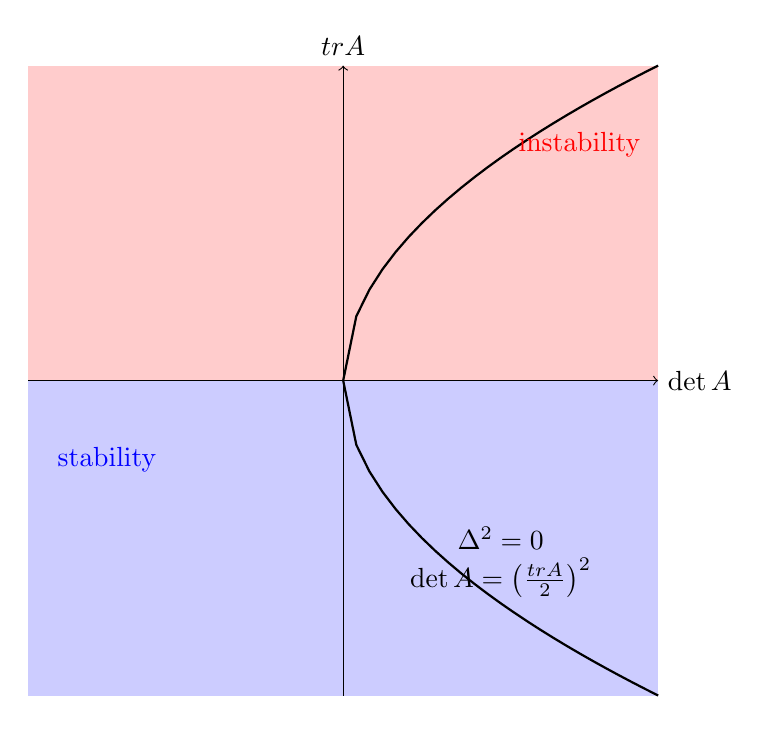
\begin{tikzpicture}
    % Set the size of the grid and the colors
    \fill[red!20] (-4,0) rectangle (4,4);
    \fill[blue!20] (-4,-4) rectangle (4,0);
    
    % Draw the axes
    \draw[->] (-4,0) -- (4,0) node[right] {$\det A$};
    \draw[->] (0,-4) -- (0,4) node[above] {$\operatorname{tr} A$};
    
    % Draw the parabola
    \draw[thick, domain=0:4] plot (\x, {sqrt(\x*4)}) node[right] {};
    \draw[thick, domain=0:4] plot (\x, {-sqrt(\x*4)}) node[right] {};
    
    % Stability and Instability regions
    \node[blue] at (-3,-1) {stability};
    \node[red] at (3,3) {instability};
    
    % Label for the critical point
    \node at (2, -2) {$\Delta^2=0$};
    \node at (2, -2.5) {$\det A = \left(\frac{\operatorname{tr} A}{2}\right)^2$};
\end{tikzpicture}

\citep{murray}


\newpage